\documentclass{standalone}
\usepackage{PhysicalChemistryNote}
\begin{document}
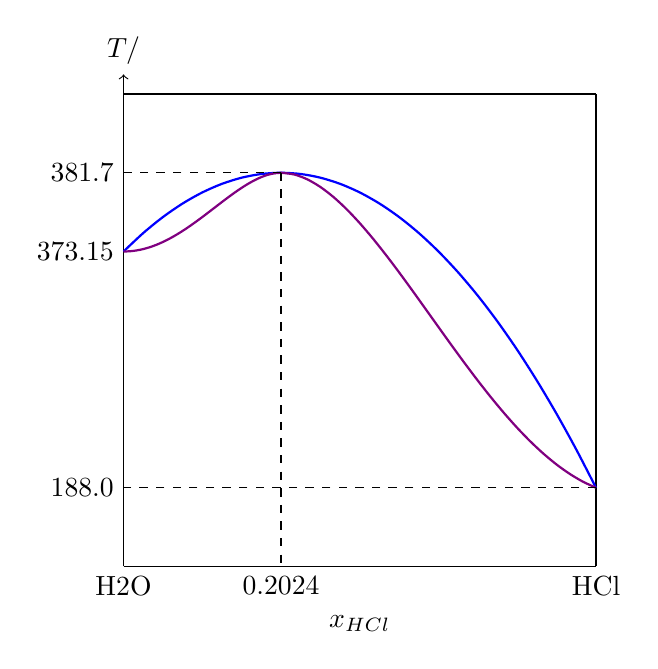
\begin{tikzpicture}
    \draw[-] (0,0) -- (6,0);
    \draw[->] (0,0) -- (0,6.25) node[above]{$T/\K$};
    \draw[-] (6,0) -- (6,6);
    \draw[-] (0,6) -- (6,6);
    \node[below] at (0,0) {{\ce{H2O}}};
    \node[below] at (6,0) {{\ce{HCl}}};
    \node[below] at (3,-0.5) {$x_{\ce{HCl}}$};
    \draw[domain=0:6,thick,blue] plot[smooth](\x,{-(\x-2)^2/4+5});
    \draw[domain=2:6,thick,violet] plot[smooth](\x,{-(\x-11)^2*(\x-2)^2/100+5});
    \draw[domain=0:2,thick,violet] plot[smooth](\x,{-(\x+2)^2*(\x-2)^2/16+5});
    \draw[dashed] (2,5)--(2,0) node[below]{$0.2024$};
    \draw[dashed] (6,1)--(0,1) node[left]{$188.0\K$};
    \draw[dashed] (2,5)--(0,5) node[left]{$381.7\K$};
    \node[left] at (0,4) {$373.15\K$};
\end{tikzpicture}
\end{document}